% Template:     Informe LaTeX
% Documento:    Archivo de ejemplo
% Versión:      7.3.7 (21/08/2021)
% Codificación: UTF-8
%
% Autor: Pablo Pizarro R.
%        Facultad de Ciencias Físicas y Matemáticas
%        Universidad de Chile
%        pablo@ppizarror.com
%
% Manual template: [https://latex.ppizarror.com/informe]
% Licencia MIT:    [https://opensource.org/licenses/MIT]

% ------------------------------------------------------------------------------
% NUEVA SECCIÓN
% ------------------------------------------------------------------------------
% Las secciones se inician con \section, si se quiere una sección sin número se
% pueden usar las funciones \sectionanum (sección sin número) o la función
% \sectionanumnoi para crear el mismo título sin numerar y sin aparecer en el índice


\section{Implementación}
\subsection{Arquitectura de la red}

Se decide utilizar un sistema basado en un DeepEncoder-Decoder. Estos sistemas, como su nombre sugiere, consisten de dos partes un encoder y un decoder.

El encoder esta formado por redes convolucionales que disminuyen la dimensionalidad de las imagenes que se ingresan hasta llegar a un cuello de botella (bottleneck). Es en este cuello de botella donde las redes convolucionales han extraído las características necesarias para codificar toda la información de la imagen en un vector multidimensional que representa la imagen de acuerdo al problema que se esta intendo resolver, por ejemplo en el problema de la de-reverberación se busca que esto vectores representen a la señal sin el efecto de la reverberación.

El decoder es simétrico al encoder, pero en vez de reducir la dimensionalidad del vector de características lo aumenta utilizando para ello el proceso de deconvolución. El decoder permite reconstruir la imagen a partir del vector de características obtenidos por el encoder.


Con ello, la idea detrás de la utilización de este tipo de redes es entregar a la entrada de la red un espectrograma de la señal reverberada, obtener los vectores de características en el bottleneck que represente la señal sin reverberación para finalmente reconstruir la imagen a partir de los vectores del bottleenck utilizando para ello módulos de de-convolución.


En este trabajo se utilizan dos arquitecturas, una U-net en la figura \ref{fig:unet} y una Late U-net en la figura \ref{fig:Late_unet}. La red U-net es una arquitectura clásica en el procesamiento de imágenes. Su particularidad radica en la existencia de conexiones residuales que van desde el encoder hacia el decoder, lo que permite traspasar información directamente de la imagen original a la reconstruida, a costa de un mayor costo a la hora de entrenar. 
La red Late reverberation supression UNET posee una conexión que conecta la salida de la UNET con el espectrograma original. De esta manera se busca que la red UNET aprenda lo que se desea eliminar del espectrograma original para generar la de reverberación.


\begin{figure}
    \centering
    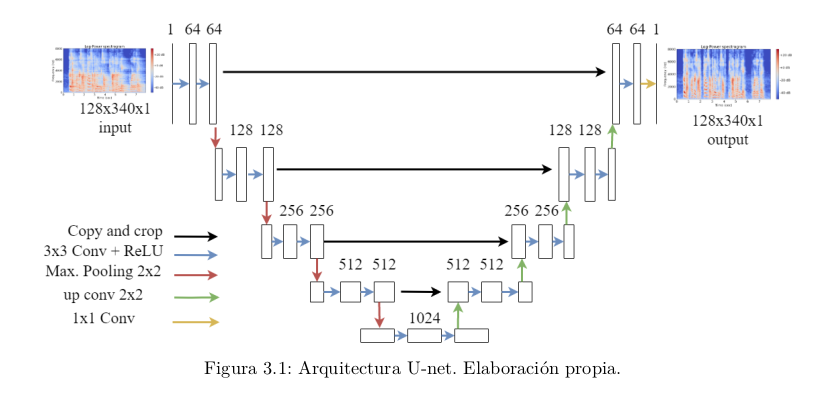
\includegraphics[scale=0.4]{img/unet.png}
    \caption{Arquitectura U-Net}
    \label{fig:unet}
\end{figure}

\begin{figure}
    \centering
    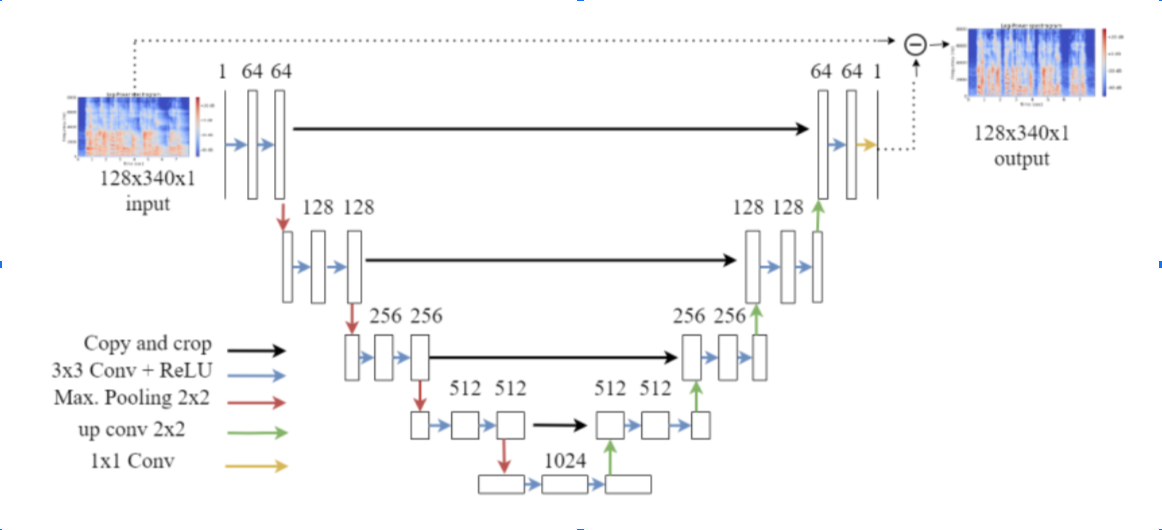
\includegraphics[scale=0.4]{img/Late_U-net.png}
    \caption{Arquitectura Late U-Net}
    \label{fig:Late_unet}
\end{figure}

\subsection{Base de datos}
Para entrenar la red se divide los 1000 pares de audios en 3 subconjuntos:
900 pares para el entrenamiento de la red, 50 para la validación del algorimo mientras se entrena y 50 pares para pruebas del sistema al finalizar el entrenamiento.

Se decide representar el audio en el espacio de frecuencia, para eso se calcula una transformada de Fourier sobre la señal de audio en el tiempo, además se utiliza una superposición de ventanas de 512, de manera que los espectrogramas poseen muestras traslapadas entre dos ventanas consecutivas.

Además se decide utilizar la escala de Mel para la representación de los intervalos de frecuencia. La escala de Mel es una escala perceptual, lo que permite comprimir la información sin degradar la percepción del sonido. En particular se utilizan 128 ceptrums para representar el espacio de frecuencias.


Aún así la duración de los audios genera espectrogramas demasiado grandes para ser procesados de manera veloz por una red, con lo que se hace un downsampling para acortar el espacio temporal del espectrograma. El resize se hace de manera que la imagen quede de 128x340 píxeles.
También es de notar que algunos audios reverberados tienen una duración mayor que la de los audios sin reebrveración, con lo que previo al resize se impone que los audios reverberados tengan igual tamaño que los audios originales.

%\begin{figure}
%    \centering
%    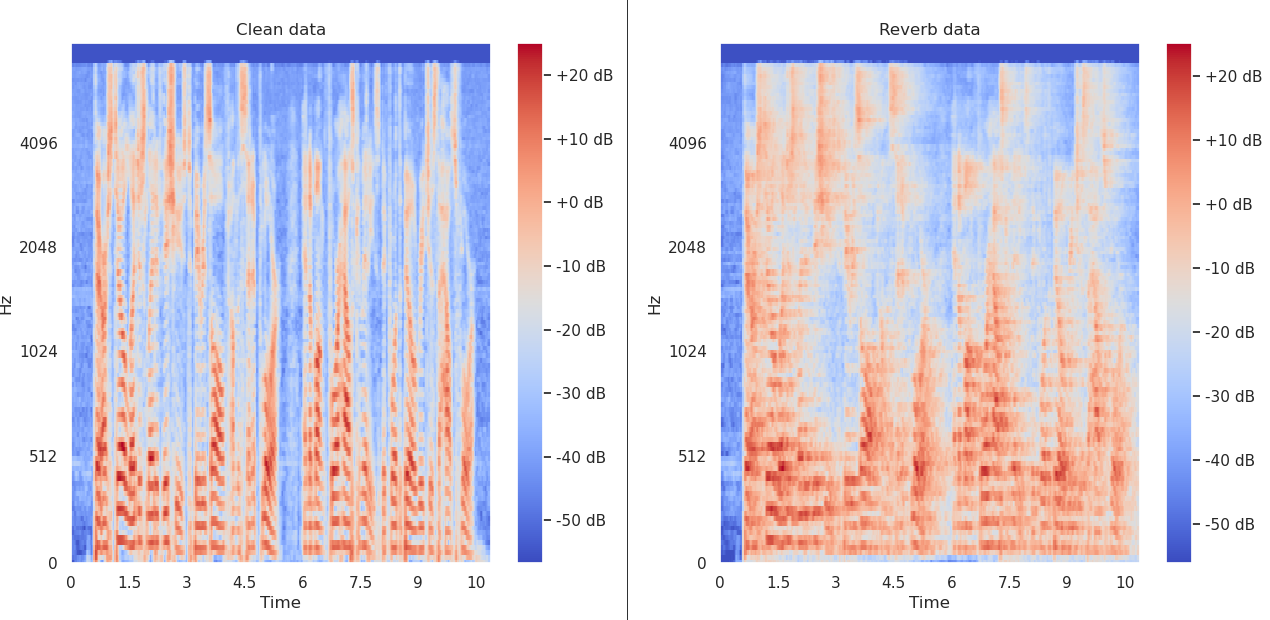
\includegraphics[scale=0.3]{img/reberv_spect.png}
%    \caption{Ejemplo par de espectrogramas limpio-reverberado.}
%    \label{fig:ex_spect}
%\end{figure}

\subsection{Reconstrucción}
Como se mencionó anteriormente la red recibe de entrada una imagen de 128x340, la procesa y entrega una imagen de 128x340 que representa el espectrograma de-reverberado. 

Para las etapas de entrenamiento se evalúa la similitud que tiene la salida de la red con el espectrograma limpio, lo que se puede hacer a nivel de imágenes por lo tanto se trabaja en el espacio de la frecuencia.

Por otro lado, a la hora de evaluar el desempeño de la red se vuelve necesario pasar la información al dominio del tiempo. Es decir se necesita hacer una transformación de un espectrograma a una señal temporal. Este no es un problema trivial, ya que un espectrograma es la representación de la magnitud que posee cada canal espectral en el tiempo, con lo que se elimina la información de fase.

Uno de los algoritmos típicamente utilizados para la transformación de espectrograma-señal temporal es el algoritmo de Griffin-Lim que permite estimar la fases de la señal si es que el espectrograma que se desea invertir posee ventanas con un overlap.


Con ello, en la etapa de pruebas del sistema se siguen los siguientes pasos:
\begin{itemize}
    \item Se hace un resize de la imagen para que recupere el tamaño que tenia previo al preprocesamiento. 
    \item Los datos se devuelven de decibelios a energía.
    \item Utilizando la librería librosa, se realiza la transformación desde Mel a audio, donde se ocupa el algoritmo Griffin-Lim para calcular la fase.
\end{itemize}

Con esto se obtienen los audios correspondientes a la salida de la red, con lo que es posible escuchar los efectos de la red sobre la reverberación.\\


Otra opción que se utilizó consististe en guardar la fase del espectrograma original, procesar la señal en la UNET y al espectrograma resultante agregarle la fase de la señal original y calcular la IFFT.


%\begin{figure}
%    \centering
%    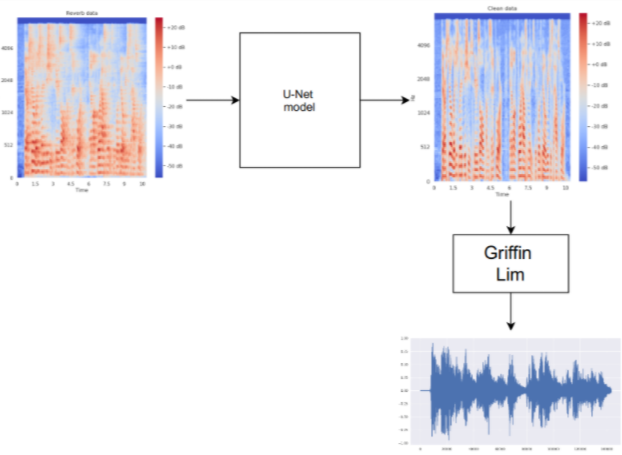
\includegraphics[scale=0.6]{img/Test_Griffin.PNG}
%    \caption{Esquema del sistema utilizando Griffin-Lim}
%    \label{fig:Griffin}
%\end{figure}
%\begin{figure}
%    \centering
%    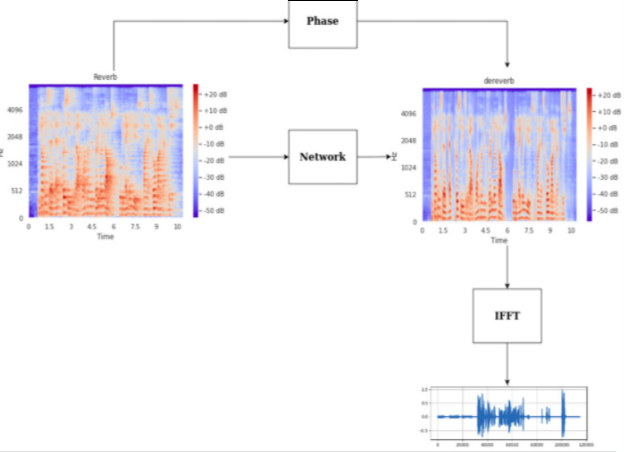
\includegraphics[scale=0.6]{img/Test_IFFT.png}
%    \caption{Esquema del sistema guardando la fase y utilizando IFFT para la reconstrucción}
%    \label{fig:IFFT}
%\end{figure}

\section{Resultados}
Las redes logran reducir el nivel de reverberación de las señales, y esto se observa claramente al comparar los espectrogramas de los audios utilizados como entrada de la red y los de salida, por ejemplo la figura \ref{fig:Spec_UNet_comp}, donde se observa claramente como el efecto de la reverberación se ve eliminada por la red U-Net, en la figura \ref{fig:Spec_LateUNet_comp} se comparan los espectrogramas de un audio sin reverberación y su versión dereverberada por la red Late U-Net, y en este caso se observa las claras similitudes de ambas imágenes, indicando un buen funcionamiento de la red, sin embargo se puede ver que las transiciones de potencia son menos suaves en el caso de la señal resultante.
Comparando los audios resultantes de ambas redes, se aprecia un mejor comportamiento en la red U-Net.\\



Sin embargo, aunque el audio resultante al final de todo el proceso es un sonido sin reberveración, este es claramente robotizado en comparación con la señal original.
El principal candidato de este efecto es el algoritmo Griffin-Lim, por lo que se realiza pruebas guardando la fase original de la señal para poder reconstruir el audio, en las figuras \ref{fig:Time_UNet_comp} y \ref{fig:Time_LateUNet_comp} se muestra las señales reconstruidas por ambos métodos para la red U-Net y Late U-Net respectivamente.


Aún con esto el sonido robótico persiste y comparando las señales resultantes de cada reconstrucción con la señal original de la figura \ref{fig:Time_OG} es notorio que pese a que mantienen formas similares existen cambios en las amplitudes y hay cambios sumamente bruscos que pueden denotar las distorsiones que genera el sistema.

Comparando el audio de ambos métodos de reconstrucción, se nota que utilizando la fase original más IFFT el resultado empeora en calidad, por lo que se prefiere el uso del método de Griffin-Lim para la reconstrucción.

Una posible opción para disminuir este comportamiento no deseado, es crear un sistema que permita separar el audio en frases o palabras, e introducir estas secciones en la red, pero sin alterar el tamaño de la imagen del espectrograma, quizás el uso del espectrograma sin alteraciones pueda mejorar los resultados de la red, y el dividir el audio en estas secciones permita el uso de la imagen completa sin la necesidad de cantidades absurdas de memoria.


\begin{figure}
    \centering
    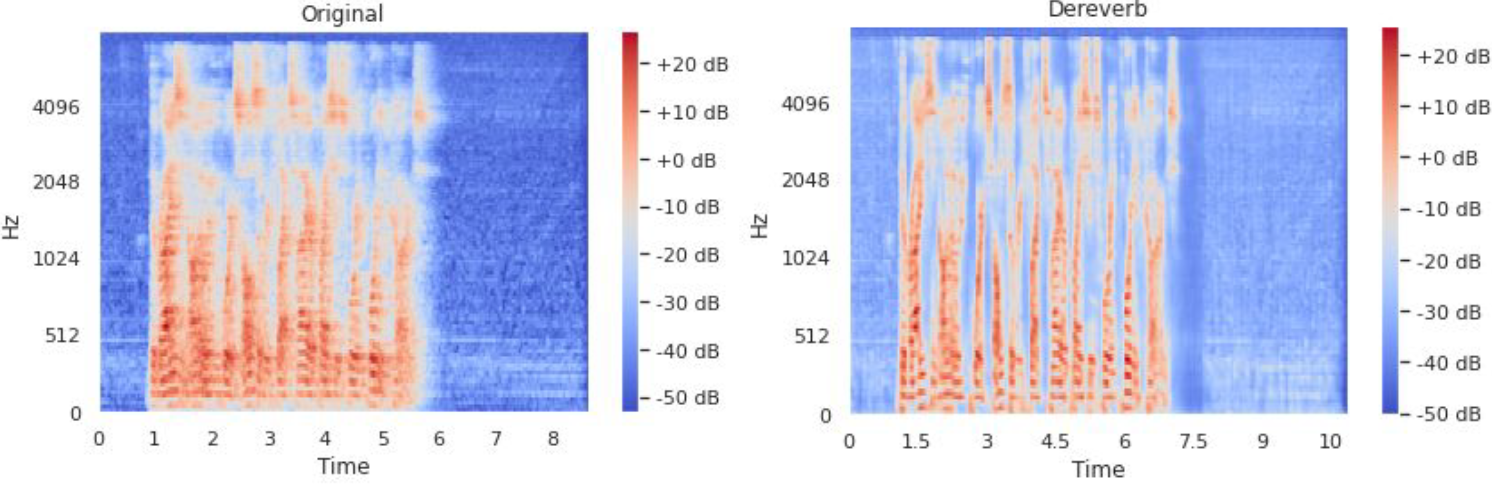
\includegraphics[scale=0.4]{img/Spect_resultados.png}
    \caption{Espectrogramas de la señal original (izquierda) y dereverberada por la red U-Net (derecha).}
    \label{fig:Spec_UNet_comp}
\end{figure}
\begin{figure}
    \centering
    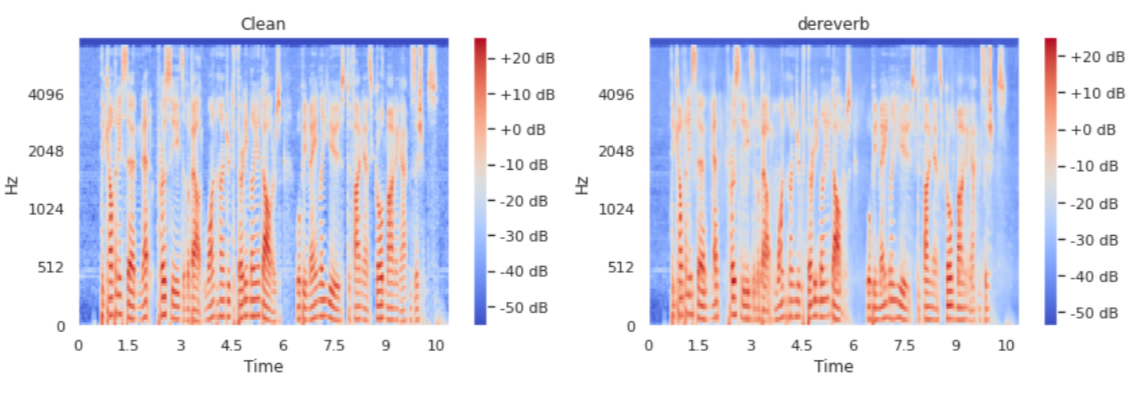
\includegraphics[scale=0.55]{img/Comp_Spect_OG-LateUNet.PNG}
    \caption{Espectrogramas de la señal original (izquierda) y dereverberada por la red Late U-Net (derecha).}
    \label{fig:Spec_LateUNet_comp}
\end{figure}

\begin{figure}
    \centering
    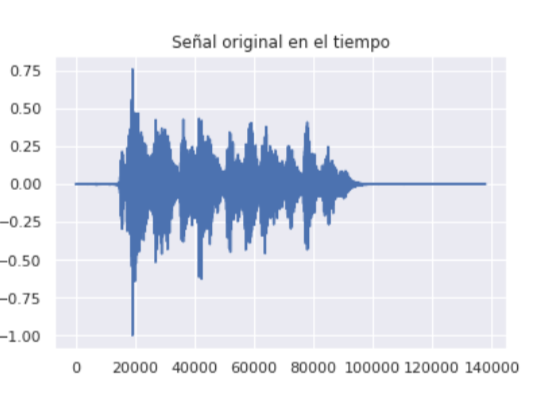
\includegraphics[scale=0.5]{img/Time_OG.png}
    \caption{Señales en el tiempo del audio original sin reverberación.}
    \label{fig:Time_OG}
\end{figure}

\begin{figure}
    \centering
    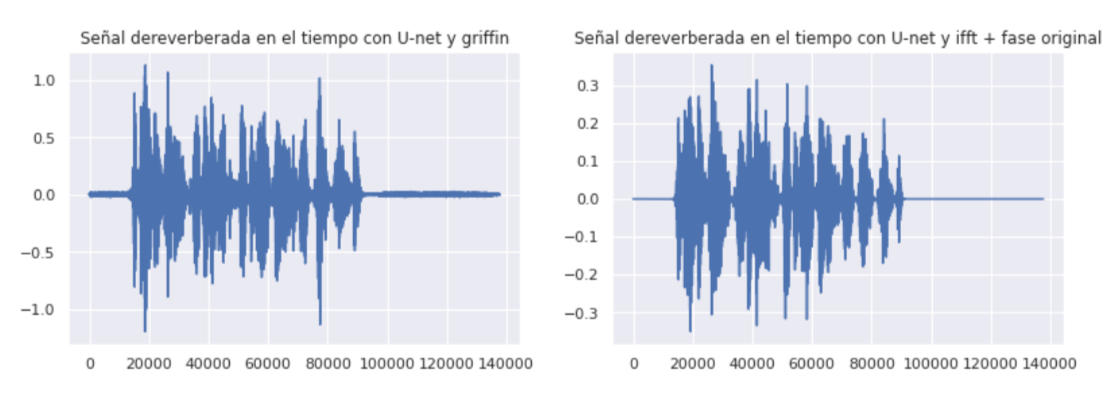
\includegraphics[scale=0.5]{img/Comp_Time_Unet.PNG}
    \caption{Señales en el tiempo de las señales de salida de la red U-Net, reconstruidas por el método de Griffin-Lim (izquierda) y fase orginal + IFFT (derecha)}
    \label{fig:Time_UNet_comp}
\end{figure}
\begin{figure}
    \centering
    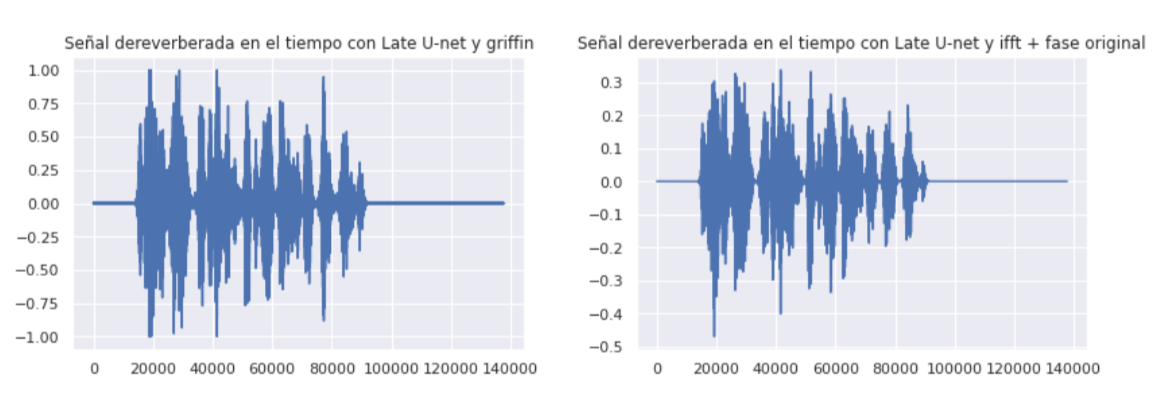
\includegraphics[scale=0.5]{img/Comp_Time_LateUnet.PNG}
    \caption{Señales en el tiempo de las señales de salida de la red Late U-Net, reconstruidas por el método de Griffin-Lim (izquierda) y fase orginal + IFFT (derecha)}
    \label{fig:Time_LateUNet_comp}
\end{figure}

\section{Conclusiones}

De este trabajo se logra obtener una red que permite dereverberar audios, con un nivel satisfactorio de efectividad. \\


Como arquitectura se utiliza una red U-Net y se le entrega los espectrogramas de la señal reverberada para trabajar como imagen, y así obtener una señal más 'limpia' que la orginal reverberada. \\


Si bien la red UNET y late UNET realizan dereverberaciones de las señales, ambos sistemas generan distorsiones en la señal temporal reconstruida. Una posible mejora a este efecto es utilizar un detector de frases o palabras de manera de dereberverar una fracción del audio de manera de eliminar el proceso de resize que puede ser uno de los causantes del efecto de robotización debido a la cuantización temporal que se utiliza.



\section*{Referencias}
[1]\emph{Diego León. 'Deconvolución en audio utilizando modelos basados en Machine Deep Learning'},2021. Disponible en http://repositorio.uchile.cl/handle/2250/181887 .\label{bib:mem_dconv}

[2] \emph{Nathanaël Perraudin, Peter Balazs, Peter L. Søndergaard. 'A fast Griffin-Lim algorithm'},2013. IEEE Workshop on Applications of Signal Processing to Audio and Acoustics, 2013, pp. 1-4.

